\cotefile{148}
\scanpage{2}

\margin{(29.11.83)}

Soit $X$ surf. à bord compacte orientée, à
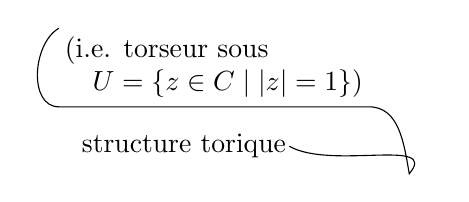
\begin{tikzpicture}[baseline=(torique.base)]
\node[anchor=west,inner sep=1pt] (torique) at (0,0) {structure torique};
\node[anchor=south west,inner sep=2pt,align=left] (torusnote) at (-.25,.5)
{\inserted{\begin{tabular}{@{}l@{}}(i.e. torseur sous\\
\quad$\mathbb U=\{z\in\mathbb C\mid |z|=1\}$)\end{tabular}}};
\draw (torusnote.north west) to[out=210,in=180] (torusnote.south west)
 -- (torusnote.south east) to[out=0,in=100] (4.2,-.35)
 to[out=50,in=-30] (torique.east);
\end{tikzpicture}
donnée sur les comp. connexes du bord.
On définit

\[
\begin{aligned}
\operatorname{SRT}(\unsure{X})={}&
\text{quotient du groupe des autom de }X
\text{ (\deleted{\unsure{en|on}} resp. l'orientation}\\
&\text{et les structures toriques) par la comp. neutre du}\\
&\text{sous-groupe }\operatorname{Aut}^!(\vec X)
\deleted{\unsure{\mathrm{bijec.}|\mathrm{diag}}}
\text{ \unsure{de|des} Aut qui induit}\\
&\text{l'identité sur }\partial X
\end{aligned}
\]

On a ainsi un dévissage de $\operatorname{SRT}(X)$ en trois étages

\[
\underbrace{S_{\unsure{*}}T^!(X)}_{
\operatorname{Aut}^!(\unsure{\vec X|\overline X})/
\text{comp. neutre}}
\qquad\mathbb U^I\qquad\unsure{\mathfrak S_I}
\qquad I=\pi_0(\partial X)
\]

ou encore

\[
\mathbb Z^I\qquad T(X)\qquad\mathbb U^I\qquad\unsure{\mathfrak S_I}
\]

En fait, on définit can! un sous-groupe
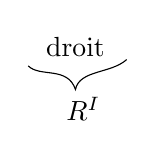
\begin{tikzpicture}[baseline=(ri.base)]
\node[inner sep=1pt] (ri) at (0,0) {$\mathbb R^I$};
\node[anchor=south] at (-.1,.55) {\inserted{droit}};
\draw (-.7,.55) .. controls (-.55,.4) and (-.2,.55) .. (-.1,.25)
 .. controls (-.05,.5) and (.35,.45) .. (.55,.63);
\end{tikzpicture}
de $\operatorname{SRT}(X)$
contenant $\mathbb Z^I$, de telle façon qu'on ait

\[
\underbrace{\operatorname{SRT}^!(X)}_{
\substack{\text{noyau de}\\
\operatorname{SRT}^!(\alpha)\to\unsure{\mathfrak S_I'|\mathfrak S_I^!}}}
=\mathbb R^I.S_*T^!(X)
\]

\diagram{
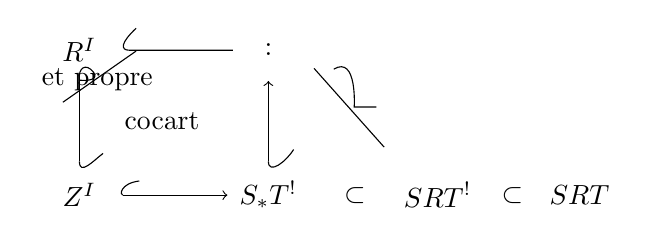
\begin{tikzpicture}[x=1cm,y=1cm]
\node (r) at (0,1.85) {$\mathbb R^I$};
\node (z) at (0,0) {$\mathbb Z^I$};
\node (p) at (2.4,1.85) {$\mathord{:}$};
\node (st) at (2.4,0) {$S_*T^!$};
\node at (3.5,0) {$\subset$};
\node at (4.55,0) {$\operatorname{SRT}^!$};
\node at (5.5,0) {$\subset$};
\node at (6.35,0) {$\operatorname{SRT}$};
\draw (.72,2.12) .. controls (.53,1.94) and (.51,1.84) .. (.64,1.84)
 -- (1.95,1.84);
% The upper end of this left stroke merges with cancelled lettering and a diagonal.
\draw (0,.43) -- (0,1.46);
\draw (0,1.46) .. controls (-.02,1.61) and (.08,1.69) .. (.18,1.56)
 .. controls (.24,1.47) and (.13,1.45) .. (0,1.46);
\draw (-.21,1.18) -- (.72,1.83);
\node[anchor=east] at (-.24,1.62) {$\unsure{\phantom{\uparrow}}$};
\draw (0,.43) .. controls (.0,.24) and (.18,.44) .. (.3,.53);
\node[anchor=west] at (.45,.94) {cocart};
\node[anchor=west] at (-.6,1.47) {\deleted{\unsure{et propre}}};
\draw[->] (.55,0) -- (1.88,0);
\draw (.76,.18) .. controls (.52,.15) and (.51,.0) .. (.55,0);
\draw[->] (2.4,.43) -- (2.4,1.45);
\draw (2.4,.43) .. controls (2.4,.25) and (2.63,.43) .. (2.72,.58);
% The following two source strokes have an unresolved reading (lambda / crossed 2).
\draw (2.98,1.61) -- (3.87,.61);
\draw (3.23,1.6) .. controls (3.53,1.78) and (3.49,1.12) .. (3.49,1.12)
 -- (3.77,1.12);
\node[anchor=west] at (3.91,1.12) {$\unsure{\phantom{\lambda}}$};
\end{tikzpicture}
}

i.e. on a

\margin{\uline{NB} $\operatorname{SUT}(X)\simeq
T(X)\times_{\unsure{\mathfrak S_I}}\operatorname{Aut}((T_i)_{i\in I})$}

\margin{Jusqu'ici on ne fait intervenir
que $S_*T^!(X)$, à l'exclusion de $S_*T(X)$,
dont la défini. exige une str. suppl.
$\uline{s}$, cf ci-dessous}

\diagram{
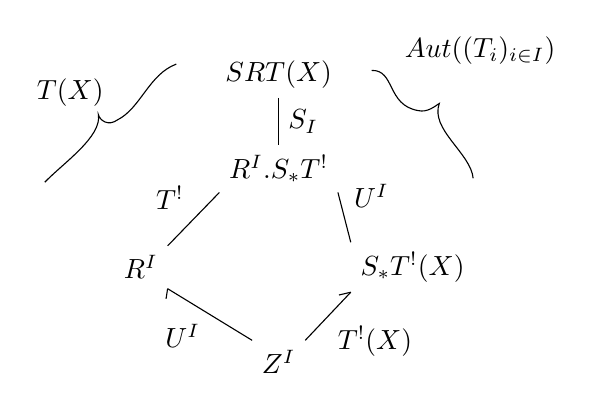
\begin{tikzpicture}[x=1cm,y=1cm]
\node (top) at (0,2.45) {$\operatorname{SRT}(X)$};
\node (mid) at (0,1.25) {$\mathbb R^I.\unsure{S_*T^!}$};
\node (left) at (-1.75,0) {$\mathbb R^I$};
\node (right) at (1.7,0) {$S_*T^!(X)$};
\node (bottom) at (0,-1.2) {$\mathbb Z^I$};
\draw (top.south) -- (mid.north) node[midway,right] {$\unsure{\mathfrak S_I}$};
\draw (mid.south west) -- (left.north east) node[midway,above left] {$T^!$};
\draw (mid.south east) -- (right.north west) node[midway,above right] {$\mathbb U^I$};
\draw (left.south east) -- (bottom.north west) node[midway,below left] {$\mathbb U^I$};
\draw (bottom.north east) -- (right.south west) node[midway,below right] {$T^!(X)$};
% Short terminal returns are drawn; their arrowhead status remains uncertain.
\draw (left.south east) -- ++(-.02,-.13);
\draw (right.south west) -- ++(-.15,-.035);
\node at (-1.24,-.4) {$\unsure{}$};
\node at (1.27,-.39) {$\unsure{}$};
\draw (-1.3,2.58) .. controls (-1.65,2.45) and (-1.75,2.02) .. (-2.05,1.87)
 .. controls (-2.16,1.79) and (-2.27,1.86) .. (-2.29,1.94)
 .. controls (-2.24,1.66) and (-2.74,1.32) .. (-2.97,1.08);
\node[anchor=east] at (-2.1,2.22) {$T(X)$};
\draw (1.18,2.5) .. controls (1.48,2.51) and (1.37,2.06) .. (1.77,1.99)
 .. controls (1.89,1.96) and (1.99,2.05) .. (2.04,2.08)
 .. controls (1.92,1.75) and (2.44,1.45) .. (2.47,1.13);
\node[anchor=south west] at (1.48,2.45) {$\operatorname{Aut}((T_i)_{i\in I})$};
\end{tikzpicture}
}

d'où
\diagram{
\begin{tikzpicture}[x=1cm,y=1cm]
\node (quot) at (0,0) {$\operatorname{SRT}\deleted{(X)}/\mathbb Z^I
 \overset{\text{déf}}=\operatorname{SUT}(X)$};
\node (prod) at (-.85,-1.1) {$T^!(X)\times\mathbb U^I$};
\draw[->] (-1.2,-.3) -- (-1.2,-.78);
\node at (1.42,-.62) {$\Big\}\ \unsure{\mathfrak S_I}$};
\draw (-3.0,-1.52) .. controls (-2.4,-1.6) and (-2.0,-1.54) .. (-1.62,-1.51)
 .. controls (-1.44,-1.71) and (-.92,-1.6) .. (-.4,-1.51)
 .. controls (.13,-1.64) and (.48,-1.64) .. (1.1,-1.45)
 .. controls (1.52,-1.41) and (1.85,-1.47) .. (2.0,-1.47);
\end{tikzpicture}
}

\[
(*)\qquad1\longrightarrow\mathbb U^I\longrightarrow
\operatorname{SUT}(X)\longrightarrow
\unsure{\deleted{\mathfrak S}T|T}(X)-1
\]

De plus, chaque fois qu'on se donne un
marquage, i.e. un pt \deleted{\unsure{de}}

\[
\uline{s}=(s_i)\in
\prod_{i\in I=\pi_0(\partial X)}
\deleted{\unsure{\mathbb U_i|(\mathbb U_i)|(T_i)}}T_i
\]

\margin{$T_i\unsure{=|:}$ comp. connexe (torique) de
$\partial X$ d'indice $i$\par\hspace{1.1cm}$\unsure{i|\varphi}$}

on trouve un plongement
\[
S_*T^{\deleted{\unsure{!}}}(X,\uline{s})\hookrightarrow\operatorname{SRT}(X)
\]
tel qu'on en \unsure{déduise|déduire}

\[
S_*T^{\deleted{\unsure{!}}}(X,\uline{s})
\mathbin{\wedge}_{\mathbb Z^I}\mathbb R^I
\simeq\operatorname{SRT}(X)
\]

\margin{1}
